\documentclass{article}

%================  CUSTOMIZATION  =================================================%

\usepackage{KjelsethReportStyle_old}

%================  METADATA  ======================================================%

\title{\fontsize{24}{36}\selectfont Elektroniske enheter og kretser\\ % Input title
Lab 02} % Line 2 of title, \\ means next line.

\author{{\ttfamily Sølve Kjelseth}} % Input your name.
% replace \ttfamily with \normalfont to make it regular font.
% (removing \ttfamily will not do this automatically.

\date{\today} % Auto updates the date, until you export it.


%================  START OF DOCUMENT  =============================================%
\begin{document}

\maketitle % Makes title front page based on the title, author and date metadata, change at the top

%================  ABSTRACT  ======================================================%
% #region
\addtocontents{toc}{\protect\setcounter{tocdepth}{0}} % Temporarily hide from TOC
\section{Abstract} % Numbered section named Abstract
This lab investigated the behaviour and characteristics of a bipolar junction transistor (BJT) in Fixed-Bias and Voltage-Divider Bias configurations.
Two circuits were used to determine the transistor current gain, denoted \(\beta\), and the behaviour of the Voltage-Divider Bias configuration.
Theoretical calculations were performed and compared with measured values.
Using the same transistor, a Voltage-Divider Bias circuit with specific requirements was designed by calculating optimal resistor values and selecting the closest commercially available components.
Measurements were then taken to evaluate the difference between the calculated circuit and actual performance.
The experiment highlights the calculations, the underlying assumptions, and the agreement between theoretical predictions and experimental observations.


\vfill % Front page footnote
This report corresponds to the second lab exercise in the course.
The report structure has been updated based on previous feedback, and further feedback is welcome to improve clarity and quality.
All materials created for this course (%
\LaTeX~sources, images, graphs, and code) are released under the open source MIT License, and available on
\linkgithub[true][0.325]{GitHub}.

\clearpage

\tableofcontents % Generate TOC
\hfill
\listoffigures % List of figures
\hfill
\listoftables % List of tables
\addtocontents{toc}{\protect\setcounter{tocdepth}{2}} % Restore TOC depth

% #endregion
%================  INTRODUCTION  ==================================================%
\section{Introduction}
% #region
Transistors are among the most commonly used components in electronic circuits. They serve as amplifiers, switches, and signal modulators.
Even the very building blocks of modern computational electronics are transistors.
One type is the bipolar junction transistor (BJT) which is explored in this experiment.
A BJT has three terminals, called the collector, base, and emitter.
It operates by controlling the collector current through the base current, with both currents exiting through the emitter.
The most important characteristic of the BJT for this experiment is its current gain, \(\beta\), which represents the ratio of collector current to base current.
In the transistor type to be used in this experiment the gain can be several hundred, resulting in very low base currents.
Understanding transistor behaviour under various resistor configurations is essential for designing circuits to specification.

The final objective of this lab is to construct a Voltage-Divider Bias BJT circuit with commercially available resistors to meet a specified design.
The first objective was to determine the transistor's \(\beta\).
For determining this, a simple Fixed-Bias BJT circuit was constructed.
Measurements were compared with calculations to verify the accuracy of the theoretical model.
The second objective was to build a Voltage-Divider Bias BJT circuit using known resistor values, and to measure and calculate its behaviour to understand how the circuit functions.
Finally, the \(\beta\) determined in the first objective and the analysis from the second objective were used to complete the final design.

This experiment demonstrates the function of a BJT and how resistor values influence circuit operation.
It also highlights the practical consideration of adapting calculated ideal values to commercially available components.

% #endregion

%================  SECTION  =======================================================%
\section{Transistor characteristics}
% #region

%================  SUBSECTION  ====================================================%
\subsection{Fixed-Bias BJT Analysis}

The first step of part 1 of the assignment is to determine the transistor's current gain \(\beta\).
The circuit shown in Figure~\ref{fig:circuit1} was constructed and the relevant measurements were recorded, summarised in Table~\ref{tab:1a}. 
From these values, the base current \(I_B\) and collector current \(I_C\) are calculated using Equations~\ref{eq:IB} and \ref{eq:IC}, respectively.
Finally, the transistor gain \(\beta\) is obtained using the results from the previous equations, as shown in Equation~\ref{eq:Beta}.

%================  SINGLE FIGURE  =================================================%
\begin{figure}[h]% Circuit 1
    \centering
    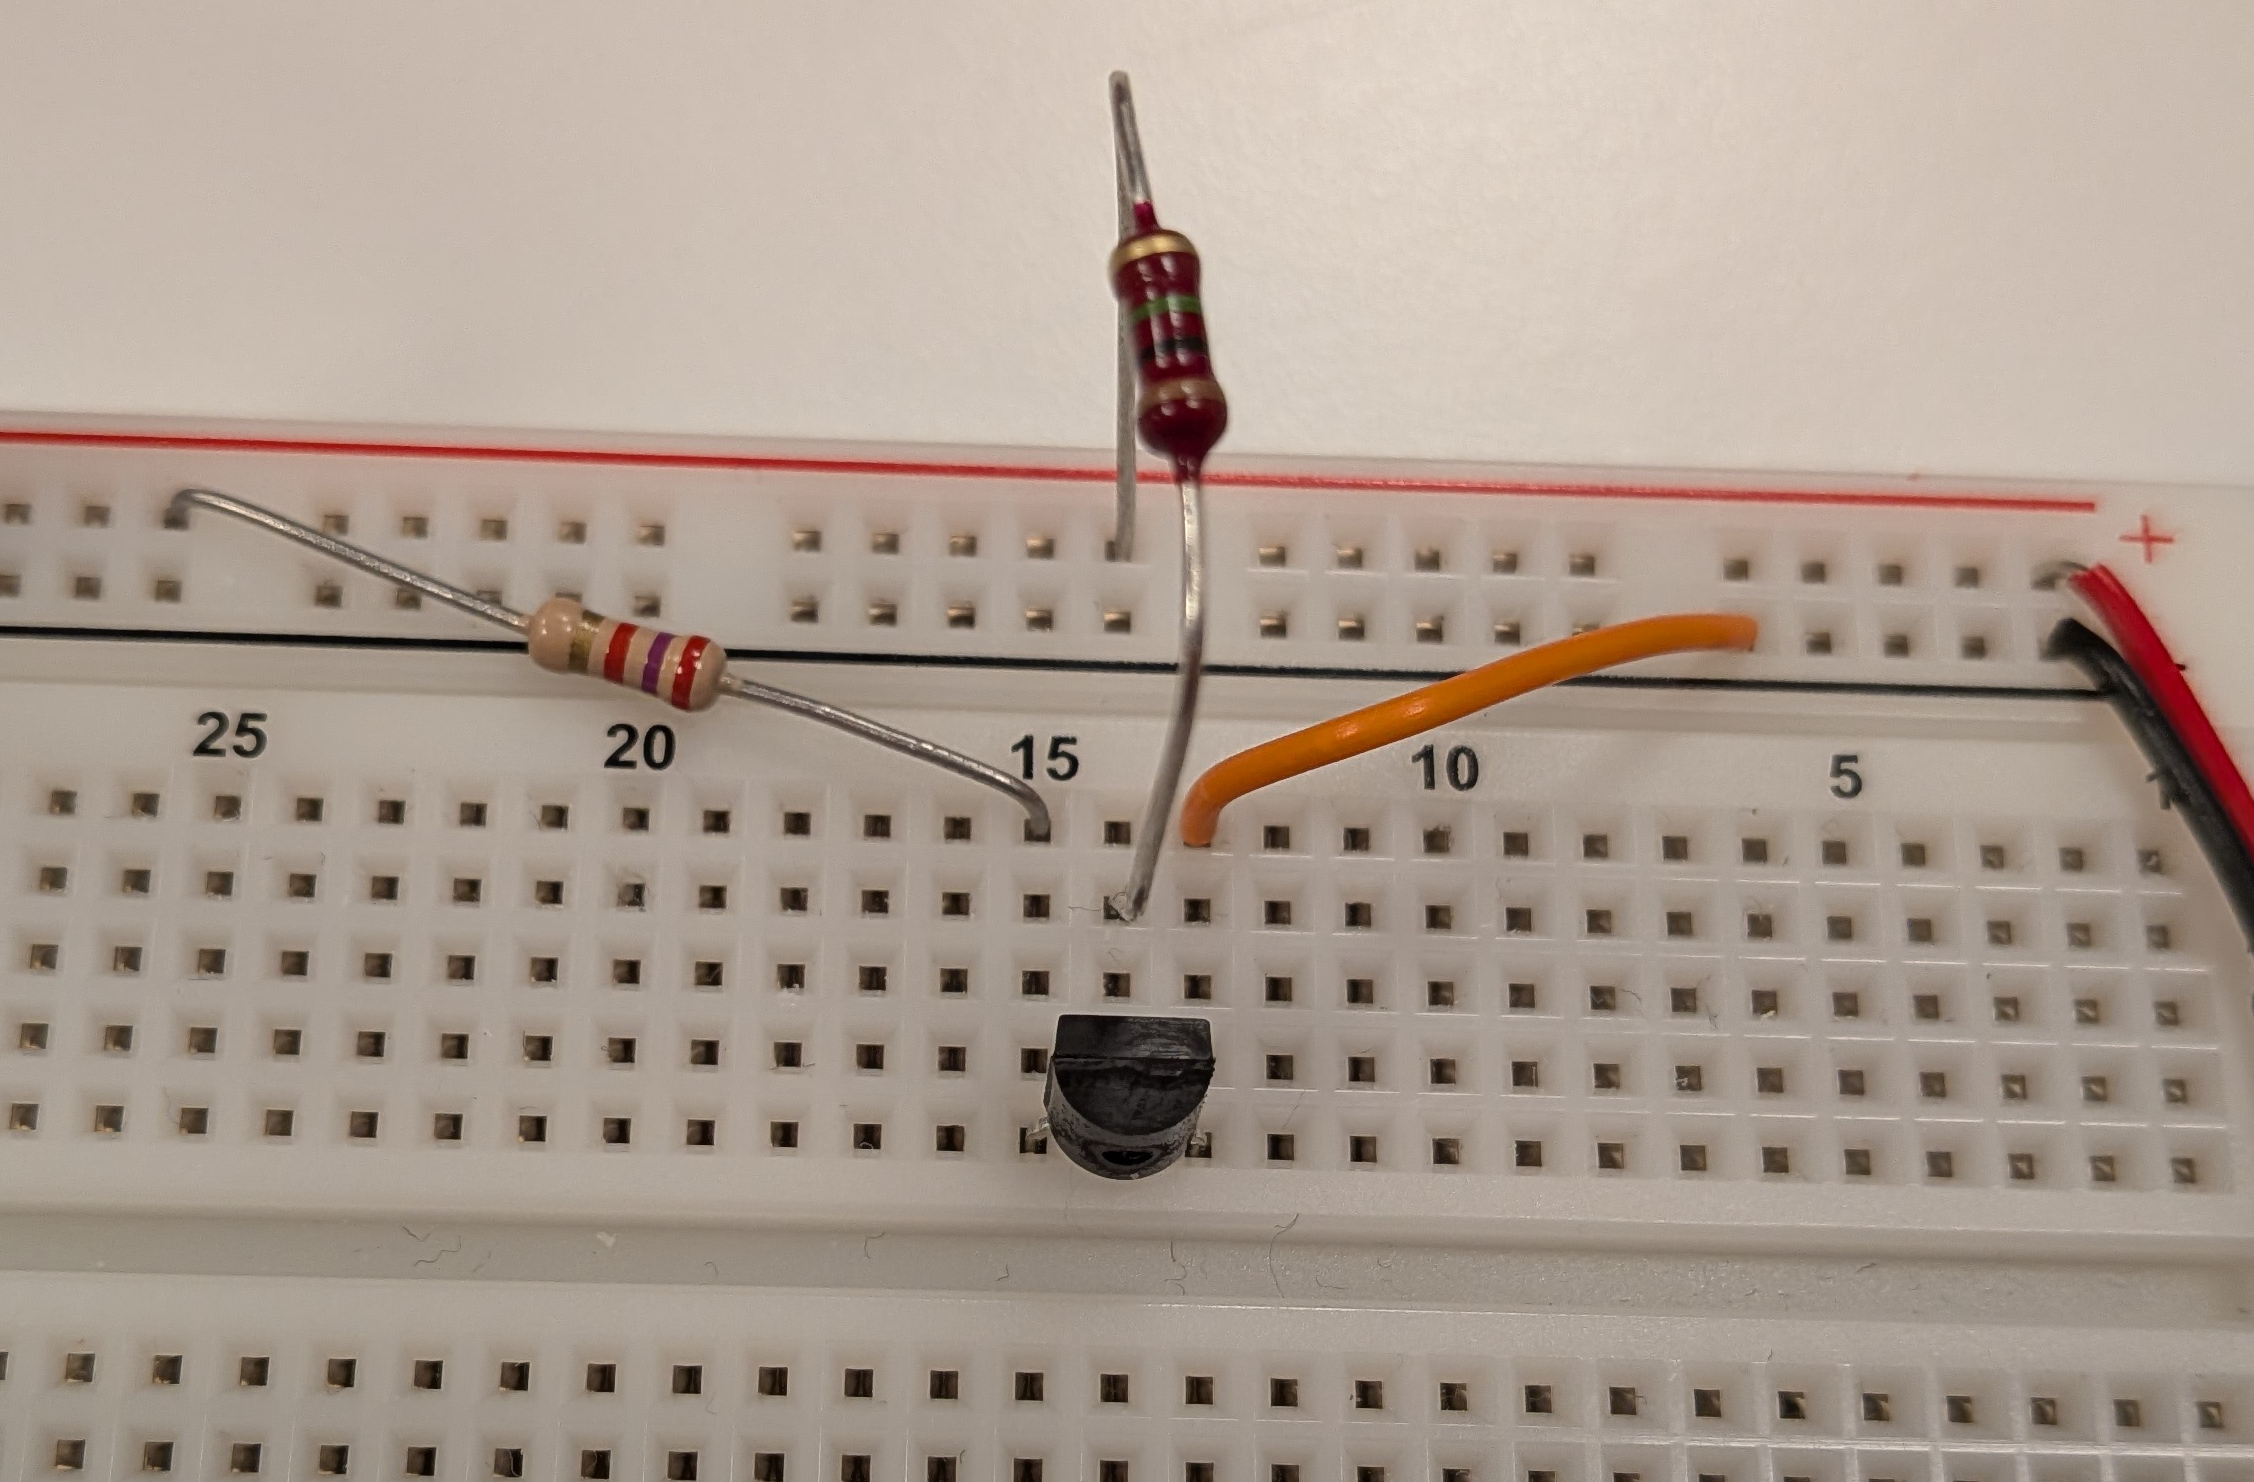
\includegraphics[width=\textwidth]{Circuit1.jpg}
    \caption{Photograph of the constructed fixed-bias BJT circuit.}
    \label{fig:circuit1}
\end{figure}

Figure~\ref{fig:circuit1} shows the physical layout of the Fixed-Bias BJT circuit.
The placement of the resistors and the transistor corresponds to the schematic provided in the assignment.
This photograph shows the actual circuit used for measurement.

%================  TABLE: MEASURED VALUES ========================================%
% Table generated by Excel2LaTeX from sheet 'Sheet1'
\begin{table}[H]% Table measurements
    \centering
    \caption{Measured values for the Fixed-Bias circuit}
    \begin{tabular}{l S[table-format=3.2] l}
        \toprule
        Parameter & {Value} & {Unit}\\
        \midrule
        \(R_B\)     & 997.80 & \si{\kilo\ohm} \\
        \(R_C\)     & 2.76   & \si{\kilo\ohm} \\
        \(V_{CC}\)  & 20.01  & \si{\volt} \\
        \(V_{BE}\)  & 0.68   & \si{\volt} \\
        \(V_{RC}\)  & 10.03  & \si{\volt} \\
        \bottomrule
    \end{tabular}%
    \label{tab:1a}%
\end{table}%

Table~\ref{tab:1a} presents the raw measurements obtained from the circuit. These values form the basis for calculating the base and collector currents.

%================  EQUATION  ======================================================%
\begin{equation}% IB
    \label{eq:IB}
    I_B = \frac{V_{CC} - V_{BE}}{R_B}
\end{equation}

%================  EQUATION  ======================================================%
\begin{equation}% IC
\label{eq:IC}
    I_C = \frac{V_{RC}}{R_C}
\end{equation}

%================  EQUATION  ======================================================%
\begin{equation}% Beta
\label{eq:Beta}
    \beta = \frac{I_C}{I_B}
\end{equation}

Equations~\ref{eq:IB}--\ref{eq:Beta} show how the base current, collector current, and transistor gain \(\beta\) are computed from the measured values.

%================  TABLE: CALCULATED VALUES =======================================%
% Table generated by Excel2LaTeX from sheet 'Sheet1'
\begin{table}[H]% Calculations
    \centering
    \caption{Calculated currents and current gain}
    \begin{tabular}{l S[table-format=3.2] l}
        \toprule
        Parameter & {Value} & {Unit} \\
        \midrule
        \(I_B\)     & 19.37    & \si{\micro\ampere} \\
        \(I_C\)     & 3.63     & \si{\milli\ampere} \\
        \(\beta\)   & 187.45   & --- \\
        \bottomrule
    \end{tabular}
    \label{tab:1d}
\end{table}

Table~\ref{tab:1d} summarizes the calculated base and collector currents, along with the resulting transistor gain.

\subsection{Voltage and Current Verification}

Part 2 begins by calculating \(I_B\) and \(I_C\) using the measured \(\beta\) and experimental data.  
This step is somewhat redundant, as the currents were already determined from the measurements, so repeating the calculation yields essentially the same values with a \(\SI{0}{\percent}\) difference. 

Next, the node voltages \(V_B\), \(V_C\), \(V_E\), and the collector-emitter voltage \(V_{CE}\) are calculated using Equations~\ref{eq:VB}--\ref{eq:VCE}.  
These calculated values are summarised in Table~\ref{tab:2b}.  
Note that \(V_E\) is directly connected to ground, so it is \(\SI{0}{\volt}\). 


%================  EQUATION  ======================================================%
\begin{equation}% VB
\label{eq:VB}
    V_B = V_{CC} - (I_B \cdot R_B)
\end{equation}


%================  EQUATION  ======================================================%
\begin{equation}% VC
\label{eq:VC}
    V_C = V_{CC} - (I_C \cdot R_C)
\end{equation}

%================  EQUATION  ======================================================%
\begin{equation}% VCE
\label{eq:VCE}
    V_{CE} = V_C - V_E
\end{equation}

Equations~\ref{eq:VB} and \ref{eq:VC} give the base and collector node voltages, obtained from the voltage drops across \(R_B\) and \(R_C\) using the corresponding currents.  
Equation~\ref{eq:VCE} defines the collector-emitter voltage as the difference between \(V_C\) and \(V_E\).  
The calculated values are summarised in Table~\ref{tab:2b}.



%================  TABLE  =========================================================%
% Table generated by Excel2LaTeX from sheet 'Sheet1'
\begin{table}[H]% Calculated
    \centering
    \caption{Calculated voltages from the circuit analysis}
    \begin{tabular}{l S[table-format=2.3] l}
        \toprule
        Parameter & {Value} & {Unit} \\
        \midrule
        \(V_B\)     & 0.684 & \si{\volt} \\
        \(V_C\)     & 9.980 & \si{\volt} \\
        \(V_E\)     & 0.000 & \si{\volt} \\
        \(V_{CE}\)  & 9.980 & \si{\volt} \\
        \bottomrule
    \end{tabular}%
    \label{tab:2b}%
\end{table}%

These calculated voltages serve as a theoretical reference for comparison with the measurements from the physical circuit.

%================  TABLE  =========================================================%
% Table generated by Excel2LaTeX from sheet 'Sheet1'
\begin{table}[H]% Measured
    \centering
    \caption{Measured voltages from the actual circuit}
    \begin{tabular}{l S[table-format=2.3] l}
        \toprule
        Parameter & {Value} & {Unit} \\
        \midrule
        \(V_B\)     & 0.683 & \si{\volt} \\
        \(V_C\)     & 9.970 & \si{\volt} \\
        \(V_E\)     & 0.000 & \si{\volt} \\
        \(V_{CE}\)  & 9.970 & \si{\volt} \\
        \bottomrule
    \end{tabular}%
    \label{tab:2c}%
\end{table}%

The measured voltages are recorded directly from the circuit.  
Comparing these with the calculated values allows assessment of the accuracy of the theoretical model.

%================  EQUATION  ======================================================%
\begin{equation}% Difference
\label{eq:diff}
    Difference = \frac{Measued - Calculated}{Calculated} \cdot 100
\end{equation}

Equation~\ref{eq:diff} defines the relative percentage difference between measured and calculated voltages, providing a quantitative measure of error.

%================  TABLE  =========================================================%
% Table generated by Excel2LaTeX from sheet 'Sheet1'
\begin{table}[H]% Difference
    \centering
    \caption{Relative difference between measured and calculated voltages}
    \begin{tabular}{l S[table-format=3.2]}
        \toprule
        Parameter & {Difference \%} \\
        \midrule
        \(V_B\)     & -0.15 \\
        \(V_C\)     & -0.10 \\
        \(V_E\)     &  0.00 \\
        \(V_{CE}\)  & -0.10 \\
        \bottomrule
    \end{tabular}%
    \label{tab:2diff}%
\end{table}%

The relative differences shown in Table~\ref{tab:2diff} confirm that the measured values closely match the theoretical predictions.  
This comparison validates the use of the measured \(\beta\) for calculating the circuit behaviour and highlights the minimal experimental error. The small error mainly reflects that measured rather than ideal theoretical values were used in the calculations.

\subsection{Voltage-Divider Bias Analysis}

Part 3 examines the behaviour of the transistor when configured with a Voltage-Divider Bias instead of the Fixed-Bias arrangement used previously.  
The constructed circuit is shown in Figure~\ref{fig:circuit2}.  
It should be noted that the photograph was taken prior to correcting a wiring error at the base connection, which was resolved before any measurements were performed.  

The resistor values were first measured, as listed in Table~\ref{tab:3a}.  
Using these, approximate voltages and currents were calculated from Equations~\ref{eq:VBapprox}--\ref{eq:VCEapprox}, with results shown in Table~\ref{tab:3b}.  
Measurements of the actual circuit were then recorded in Table~\ref{tab:3c}, and the calculated and measured results were compared. 
The outcome of this comparison is presented in Table~\ref{tab:3diff}, allowing an evaluation of how closely the theoretical model matches the real circuit.  


%================  SINGLE FIGURE  =================================================%
\begin{figure}[h]% Circuit 2
\centering
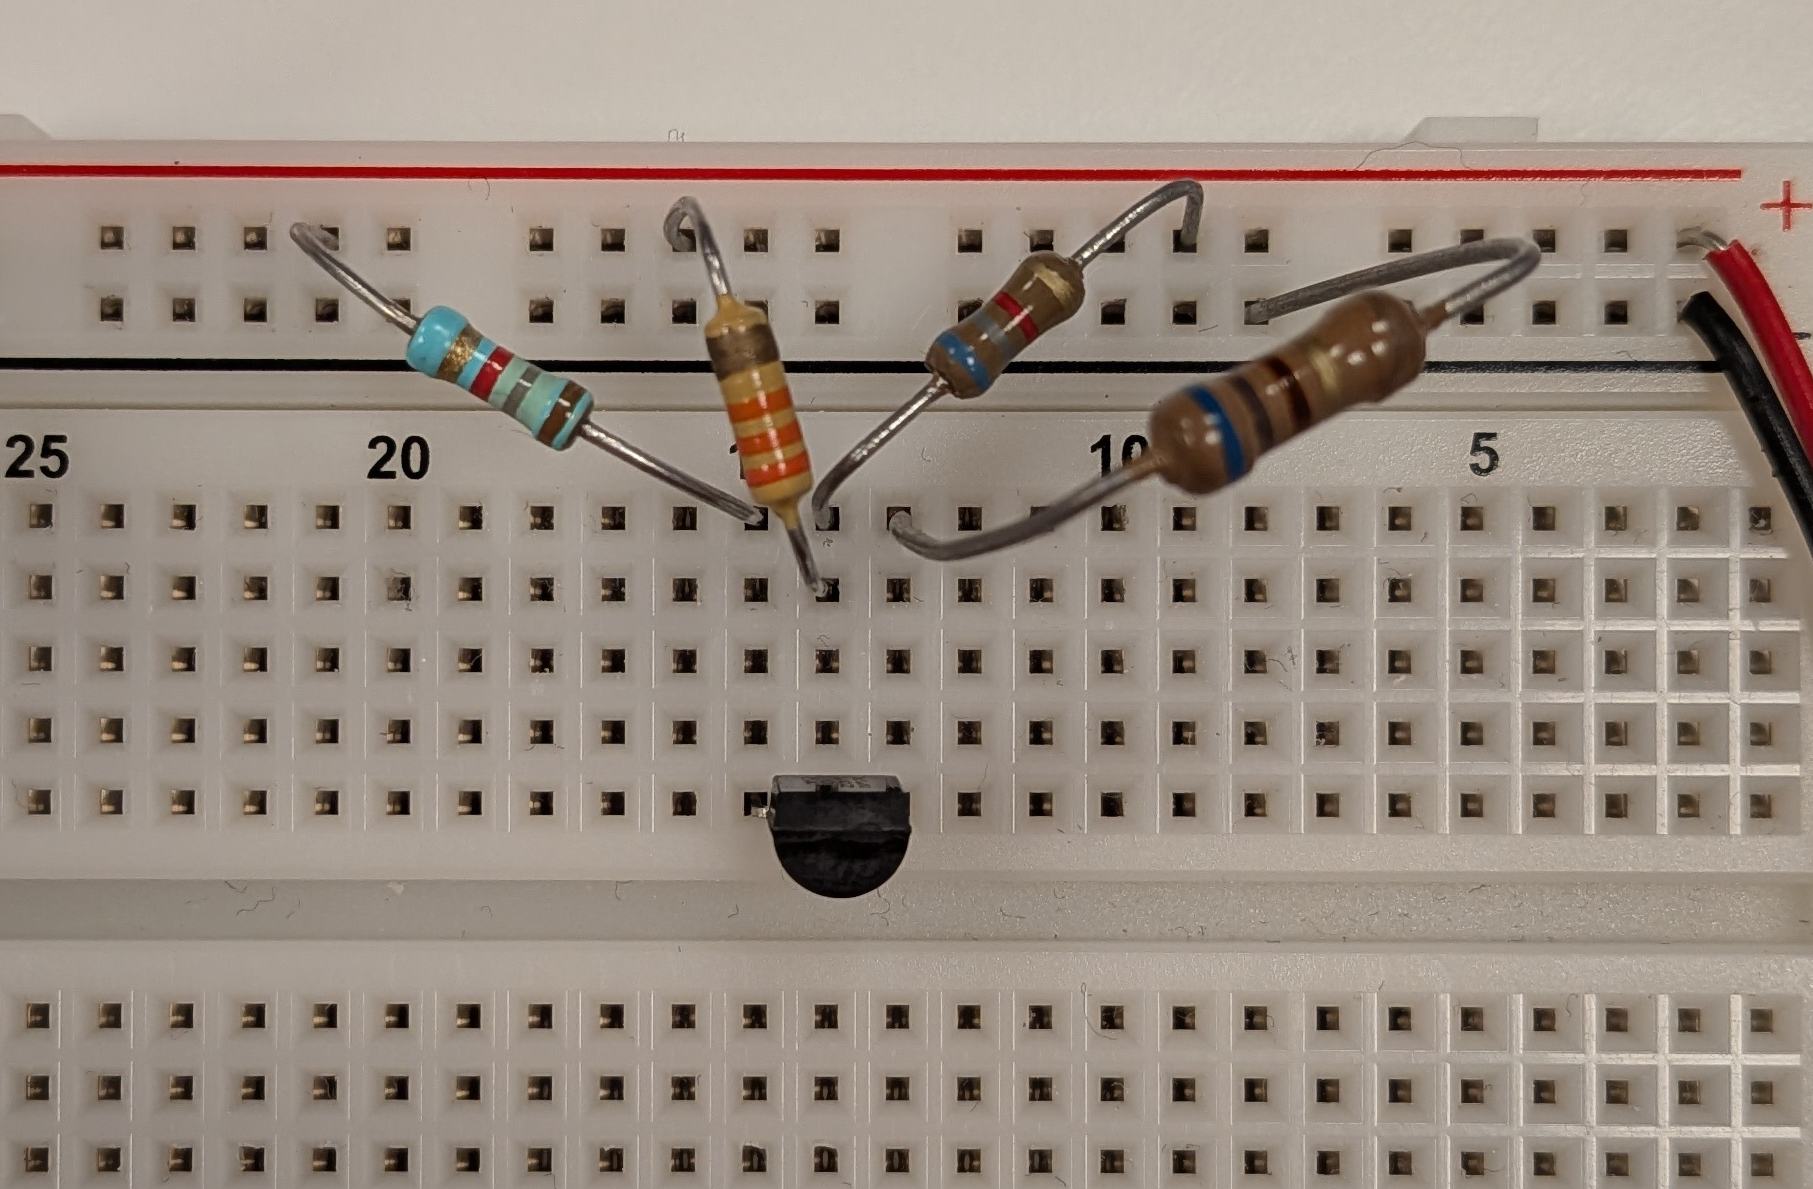
\includegraphics[width=\textwidth]{Circuit2.jpg}
\caption{Photograph of the (incorrectly connected) Voltage-Divider Bias BJT circuit.}
\label{fig:circuit2}
\end{figure}

The resistor values of the circuit were first measured, and these results are summarised in Table~\ref{tab:3a}.  
These measurements are used as the basis for the subsequent theoretical calculations. 

%================  TABLE  =========================================================%
% Table generated by Excel2LaTeX from sheet 'Sheet1'
\begin{table}[H]% Resistances
  \centering
  \caption{Measured resistance values for the Voltage-Divider Bias circuit}
    \begin{tabular}{l S[table-format=3.3] l}
    \toprule
    Parameter & {Value} & {Unit} \\
    \midrule
    \(R_1\) & 33.868    & \si{\kilo\ohm} \\
    \(R_2\) & 6.825     & \si{\kilo\ohm} \\
    \(R_C\) & 1.799     & \si{\kilo\ohm} \\
    \(R_E\) & 675.400   & \si{\ohm} \\
    \bottomrule
    \end{tabular}%
  \label{tab:3a}%
\end{table}%

From these resistance values, the node voltages and corresponding current values are estimated, along with the collector-emitter voltage drop, using Equations~\ref{eq:VBapprox}--\ref{eq:VCEapprox}.

%================  EQUATION  ======================================================%
\begin{equation}% VB
\label{eq:VBapprox}
    V_B \approx V_{CC} \cdot \frac{R_2}{R_1 + R_2}
\end{equation}

Equation~\ref{eq:VBapprox} provides an approximate value of the base voltage, assuming that the base current \(I_B\) is negligible compared with the current through \(R_2\).  

%================  EQUATION  ======================================================%
\begin{equation}% VE
\label{eq:VEapprox}
    V_E = V_B - V_{BE}
\end{equation}

Equation~\ref{eq:VEapprox} gives the emitter voltage as the difference between the base voltage and the base-emitter drop, where \(V_{BE}\) is assumed to be \(\SI{0.7}{\volt}\).  


%================  EQUATION  ======================================================%
\begin{equation}% IE
\label{eq:IEapprox}
    I_E = \frac{V_E}{R_E}
\end{equation}

Equation~\ref{eq:IEapprox} relates the emitter current to the emitter voltage and the emitter resistance.  


%================  EQUATION  ======================================================%
\begin{equation}% IB
\label{eq:IBapprox}
    I_B = \frac{I_E}{\beta + 1}
\end{equation}

%================  EQUATION  ======================================================%
\begin{equation}% IC
\label{eq:ICapprox}
    I_C = I_B \cdot \beta
\end{equation}

Equations~\ref{eq:IBapprox} and \ref{eq:ICapprox} determine the base and collector currents from the emitter current and the transistor gain \(\beta\).  
The value of \(\beta\) was obtained experimentally in Part 1 (Equation~\ref{eq:Beta}) and has been applied throughout these calculations.  
 

%================  EQUATION  ======================================================%
\begin{equation}% VC
\label{eq:VCapprox}
    V_C = V_{CC} - (I_C \cdot R_C)
\end{equation}

Equation~\ref{eq:VCapprox} calculates the collector node voltage from the supply voltage and the voltage drop across the collector resistor.  


%================  EQUATION  ======================================================%
\begin{equation}% VCE
\label{eq:VCEapprox}
    V_{CE} = V_C - V_E
\end{equation}

Finally, Equation~\ref{eq:VCEapprox} defines the collector-emitter voltage drop as the difference between the collector and emitter node voltages.  

The values obtained from these calculations are presented in Table~\ref{tab:3b}.  

%================  TABLE  =========================================================%
% Table generated by Excel2LaTeX from sheet 'Sheet1'
\begin{table}[H]% Calculations
    \centering
    \caption{Calculated voltages and currents for the Voltage-Divider Bias circuit}
    \begin{tabular}{l S[table-format=2.3] l}
        \toprule
        Parameter & {Value} & {Unit} \\
        \midrule
        \(V_B\)     & 3.356     & \si{\volt} \\
        \(V_E\)     & 2.656     & \si{\volt} \\
        \(V_C\)     & 12.973    & \si{\volt} \\
        \(V_{CE}\)  & 10.317    & \si{\volt} \\
        \(I_E\)     & 3.933     & \si{\milli\ampere} \\
        \(I_C\)     & 3.912     & \si{\milli\ampere} \\
        \(I_B\)     & 20.868    & \si{\micro\ampere} \\
        \bottomrule
    \end{tabular}%
    \label{tab:3b}%
\end{table}%

Table~\ref{tab:3b} summarises the theoretical values of the node voltages, collector-emitter voltage, and transistor currents derived from the Voltage-Divider Bias model.  

Direct measurements of the constructed circuit were then taken, and the results are listed in Table~\ref{tab:3c}.  

% Table generated by Excel2LaTeX from sheet 'Sheet1'
\begin{table}[H]% Measurements
    \centering
    \caption{Measured voltages and currents for the Voltage-Divider Bias circuit}
    \begin{tabular}{l S[table-format=2.3] l}
        \toprule
        Parameter & {Value} & {Unit} \\
        \midrule
        \(V_B\)     & 3.239     & \si{\volt} \\
        \(V_E\)     & 2.557     & \si{\volt} \\
        \(V_C\)     & 13.230    & \si{\volt} \\
        \(V_{CE}\)  & 10.670    & \si{\volt} \\
        \(I_E\)     & 3.790     & \si{\milli\ampere} \\
        \(I_C\)     & 3.770     & \si{\milli\ampere} \\
        \(I_B\)     & 20.100    & \si{\micro\ampere} \\
        \bottomrule
    \end{tabular}%
    \label{tab:3c}%
\end{table}%

Table~\ref{tab:3c} presents the measured values obtained directly from the circuit.  
Comparing these with the calculated values provides an indication of the accuracy of the theoretical model.  

The relative percentage differences between measured and calculated results were determined using Equation~\ref{eq:diff}, which was introduced in Part 2.  
These differences are summarised in Table~\ref{tab:3diff}.  

% Table generated by Excel2LaTeX from sheet 'Sheet1'
\begin{table}[H]% Difference
    \centering
    \caption{Relative difference between measured and calculated values}
    \begin{tabular}{l S[table-format=3.3]}
        \toprule
        Parameter & {Difference \%} \\
        \midrule
        \(V_B\)     & -3.488 \\
        \(V_E\)     & -3.730 \\
        \(V_C\)     &  1.982 \\
        \(V_{CE}\)  &  3.424 \\
        \(I_E\)     & -3.626 \\
        \(I_C\)     & -3.623 \\
        \(I_B\)     & -3.681 \\
        \bottomrule
    \end{tabular}%
    \label{tab:3diff}%
\end{table}%

Table~\ref{tab:3diff} confirms that the measured values agree closely with the theoretical predictions.  
All differences remain within a few percent, indicating that the simplifying assumptions used in the calculations, such as neglecting the small effect of \(I_B\) in Equation~\ref{eq:VBapprox}, are justified.  
This shows that the Voltage-Divider Bias model provides a reliable representation of the actual circuit behaviour.  

The results from Parts 1 to 3 demonstrate how transistor biasing circuits can be analysed through a combination of measurement and theoretical calculation.  
The experiments confirmed that the approximate models, while simplified, provide results that agree closely with practical measurements, with only small deviations caused by component tolerances and non-ideal device behaviour.   

These findings provide a foundation for moving beyond analysis of given circuits toward the design of new ones.  
By understanding how resistor networks establish bias points and how well theoretical values align with measured results, it becomes possible to select component values that achieve desired operating conditions even under real-world constraints.  

% #endregion

%================  SECTION  =======================================================%
\section{Designing a circuit}
% #region

Part 4 shifted from analysis of provided circuits to the design of a new Voltage-Divider Bias BJT circuit that meets specific operating conditions. The design process involves calculating theoretical resistor values, selecting the nearest commercially available components, constructing the circuit, and finally comparing the measured performance with the specified targets.

The specifications are summarised in Table~\ref{tab:4specs}, the only note is that one of the specifications is calculated in the table, where in the assignment it was specified as \(V_E = 0.1 \cdot V_{CC}\).

\begin{table}[H]
    \centering
    \caption{Specifications for the circuit}
    \begin{tabular}{l S[table-format=3.3] l}
        \toprule
        Parameter & {Value} & {Unit} \\
        \midrule
        \(V_{CC}\)  & 15     & \si{\volt} \\
        \(V_{CE}\)  & 7.5    & \si{\volt} \\
        \(I_C\)     & 5      & \si{\milli\ampere} \\
        \(V_E\)     & 1.5    & \si{\volt} \\
        \bottomrule
    \end{tabular}%
    \label{tab:4specs}%
\end{table}%


The design began with calculating the collector resistor \(R_C\) using Equation~\ref{eq:RC}.



%================  EQUATION  ======================================================%
\begin{equation}
    \label{eq:RC}
    R_C = \frac{V_{R_C}}{I_C} = \frac{V_{CC} - V_{CE} - V_E}{I_C}
\end{equation}

The calculated value of \(R_C\) is \SI{1.2}{\kilo\ohm}.  
The closest commercial value of \SI{1.2}{\kilo\ohm} was chosen.

Next, the emitter resistor \(R_E\) is determined using Equation~\ref{eq:RE}, where \(I_E \approx I_C\).

%================  EQUATION  ======================================================%
\begin{equation}
    \label{eq:RE}
    R_E = \frac{V_E}{I_E} \approx \frac{V_E}{I_C}
\end{equation}

The calculated \(R_E\) is \SI{300}{\ohm}.  
A commercial resistor of \SI{270}{\ohm} was selected.
This value is preferred over \SI{330}{\ohm} because the real emitter current \(I_E\) will be slightly larger than \(I_C\) due to the base current \(I_B\), meaning the calculated value of \SI{300}{\ohm} slightly overestimates the ideal resistor.  
Choosing \SI{270}{\ohm} ensures that the actual \(R_E\) is closer to the design specification.  

The base voltage approximation is set using the voltage-divider formed by \(R_1\) and \(R_2\) as done in Equation~\ref{eq:VBapprox}.
For the voltage-divider approximation to be valid, the inequality \(\beta \cdot R_E > 10 \cdot R_2\) must be satisfied, ensuring that the base current drawn by the transistor has minimal effect on the voltage at the base.  
\(V_B\) can be expressed as the sum of emitter voltage and the base-emitter voltage drop as seen in Equation~\ref{eq:VBVEVBE}.

%================  EQUATION  ======================================================%
\begin{equation}
    \label{eq:VBVEVBE}
    V_B = V_E + V_{BE} \approx V_E + \SI{0.7}{\volt}
\end{equation}

Assuming the value of \SI{0.7}{\volt} for the base-emitter voltage drop and combining with Equation~\ref{eq:VBapprox}, an expression with only \(R_1\) and \(R_2\) as not known quantities can be made, as shown in Equation~\ref{eq:R1R2}.
This can then be rewritten to find the ratio between \(R_1\) and \(R_2\) in Equation~\ref{eq:R1R2ratio}.

%================  EQUATION  ======================================================%
\begin{equation}
    \label{eq:R1R2}
    V_E - \SI{0.7}{\volt} \approx V_{CC} \cdot \frac{R_2}{R_1 + R_2}
\end{equation}

%================  EQUATION  ======================================================%
\begin{equation}
    \label{eq:R1R2ratio}
    \frac{R_1}{R_2} = \frac{V_{CC}}{V_E + V_{BE}} - 1 = \frac{12.8}{2.2} \approx 5.\overline{81}
\end{equation}

The maximum value of \(R_2\) is found by solving the inequality that validates the voltage-divider model as shown in Equation~\ref{eq:R2max}.

%================  EQUATION  ======================================================%
\begin{equation}
    \label{eq:R2max}
    R_2 \le \frac{\beta \cdot R_E}{10}
\end{equation}

The resulting maximum value of \(R_2\) is \SI{5.061}{\kilo\ohm}.
The closest commercial value, less than this is \SI{4.7}{\kilo\ohm} and is the one selected for \(R_2\). 
Using the ratio from Equation~\ref{eq:R1R2ratio} and the chosen value for \(R_2\), \(R_1\) is calculated as seen in Equation~\ref{eq:R1_calc}.

%================  EQUATION  ======================================================%
\begin{equation}
    \label{eq:R1_calc}
    R_1 = R_2 \cdot \frac{12.8}{2.2}
\end{equation}

The calculated value for \(R_1\) is \SI{27.345}{\kilo\ohm} and the nearest commercial value of \SI{27}{\kilo\ohm} was selected to be used for \(R_1\).
A summary of all calculated and chosen values is found in Table~\ref{tab:4res} 


%================  TABLE: Calculated and chosen resistor values ========================================%
\begin{table}[H]
    \centering
    \caption{Calculated and chosen resistor values for the designed circuit}
    \begin{tabular}{l S[table-format=2.3] S[table-format=2.3] l}
        \toprule
        Parameter & {Calculated} & {Chosen} & {Unit} \\
        \midrule
        \(R_C\) & 1.200 & 1.200 & \si{\kilo\ohm} \\
        \(R_E\) & 0.300 & 0.270 & \si{\kilo\ohm} \\% Wanted to display in ohm but 
        \(R_2\) & 5.061 & 4.700 & \si{\kilo\ohm} \\% did not look good in table
        \(R_1\) & 27.345 & 27.000 & \si{\kilo\ohm} \\
        \bottomrule
    \end{tabular}
    \label{tab:4res}
\end{table}

The circuit was then constructed using the chosen resistor values as shown in Figure~\ref{fig:circuit3}.

%================  SINGLE FIGURE  =================================================%
\begin{figure}[H]
    \centering
    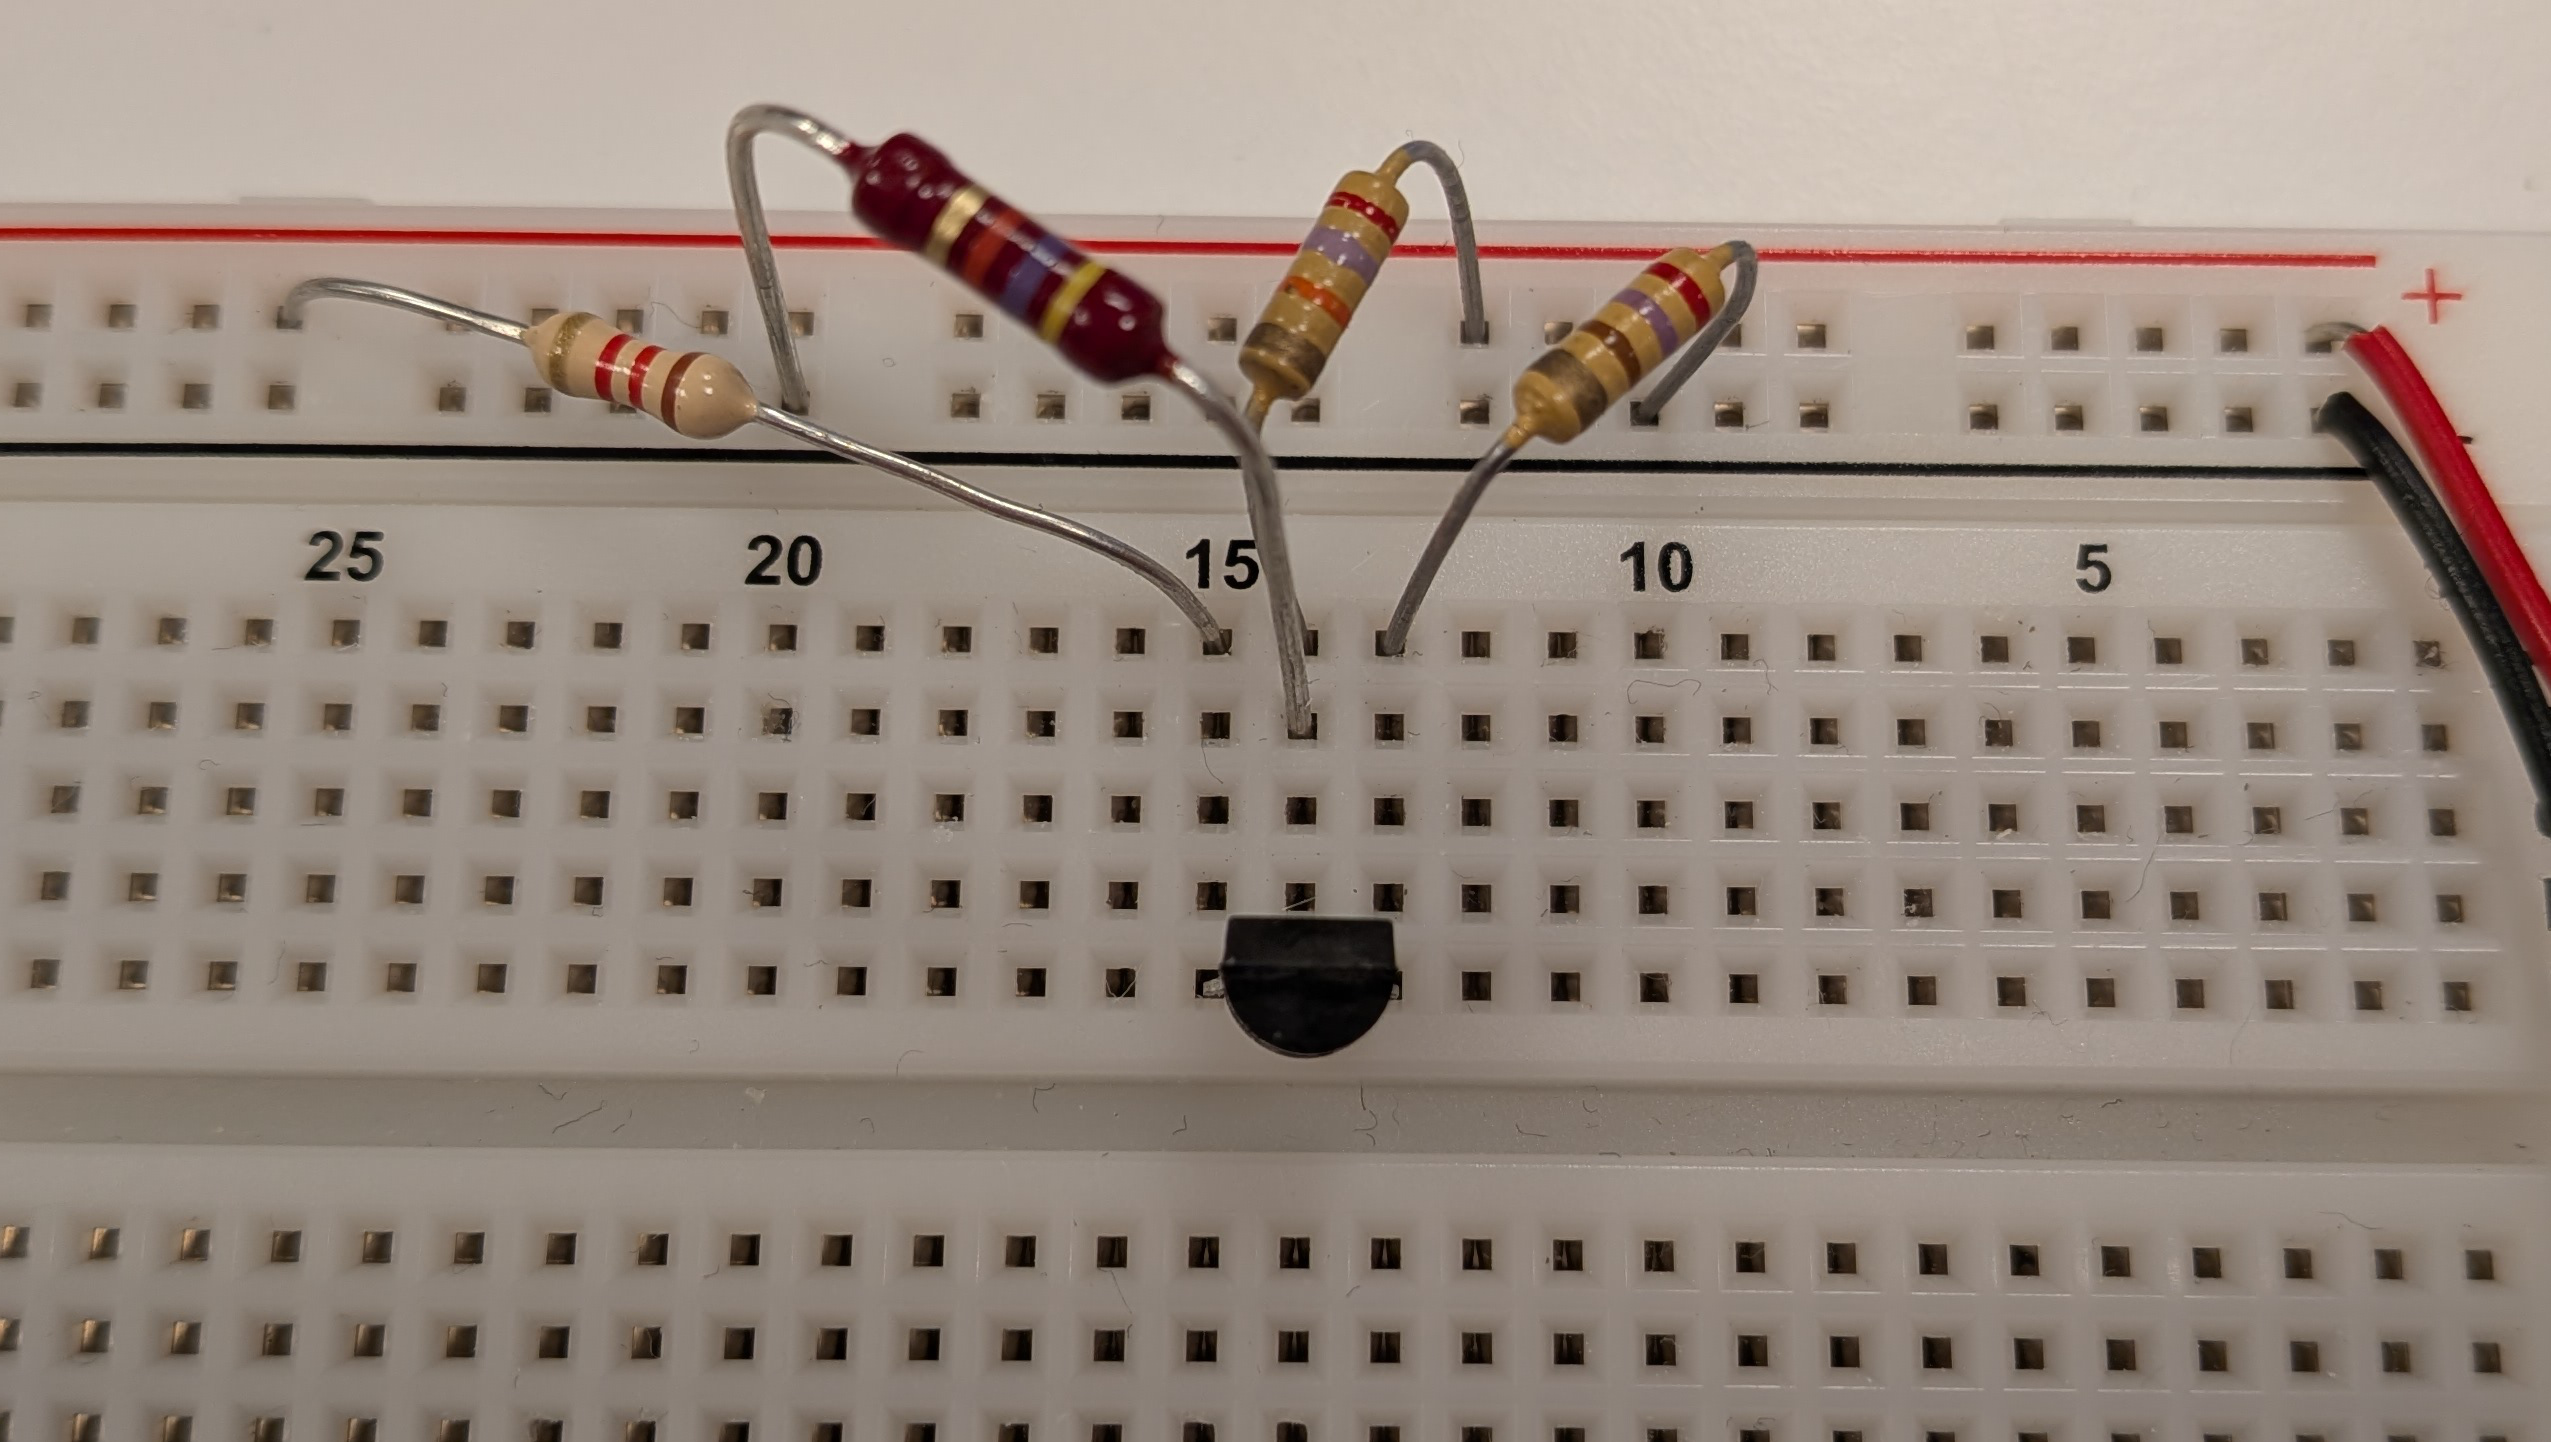
\includegraphics[width=\textwidth]{Circuit3.jpg}
    \caption{Voltage-Divider Bias BJT circuit constructed to specification.}
    \label{fig:circuit3}
\end{figure}

The voltage over \(R_C\) and its resistance is measured. Then using these values the current \(I_C\) is calculated as shown in Equation~\ref{eq:ICfinal}

%================  EQUATION  ======================================================%
\begin{equation}
    \label{eq:ICfinal}
    I_C = \frac{V_{R_C}}{R_C}
\end{equation}


Voltages across \(R_1\) and \(R_2\) and the resistor values were measured accurately.
Using the measured values, the divider currents are calculated in Equation~\ref{eq:divider}.

%================  EQUATION  ======================================================%
\begin{equation}
    \label{eq:divider}
    I_1 = \frac{V_{R_1}}{R_1}, \quad
    I_2 = \frac{V_{R_2}}{R_2}
\end{equation}

Using the values for the divider currents from Equation~\ref{eq:divider}, the base current can be calculated as shown in Equation~\ref{eq:base}.

%================  EQUATION  ======================================================%
\begin{equation}
\label{eq:base}
I_B = I_2 - I_C
\end{equation}

When both the base and collector currents are known, the \(\beta\) can be calculated the same way as in part 1, using Equation~\ref{eq:Beta}.
The emitter voltage \(V_E\) is also calculated from taking the measured supply voltage subtracting the voltage drops \(V_{R_C}\) and \(V_{CE}\) as shown in Equation~\ref{eq:VEcalc}.

%================  EQUATION  ======================================================%
\begin{equation}
\label{eq:VEcalc}
V_E = V_{CC} - V_{R_C} - V_{CE}
\end{equation}

All the measured values, and the calculated values that are based on measurements can be found summarised in Table~\ref{tab:4measured}

%================  TABLE: Measurements ========================================%
\begin{table}[H]
    \centering
    \caption{Measurements for the designed circuit}
    \begin{tabular}{l S[table-format=3.3] l}
        \toprule
        Parameter & {Value} & {Unit} \\
        \midrule
        \(R_C\)     & 1.186  & \si{\kilo\ohm} \\
        \(R_E\)     & 0.273  & \si{\kilo\ohm} \\
        \(R_1\)     & 27.306 & \si{\kilo\ohm} \\
        \(R_2\)     & 4.679  & \si{\kilo\ohm} \\
        \(V_{CC}\)  & 15.06  & \si{\volt} \\
        \(V_{R_C}\) & 6.00   & \si{\volt} \\
        \(V_{CE}\)  & 7.64   & \si{\volt} \\
        \(V_E\)     & 1.42   & \si{\volt} \\
        \(V_{R_1}\) & 12.96  & \si{\volt} \\
        \(V_{R_2}\) & 2.093  & \si{\volt} \\
        \(I_C\)     & 5.078  & \si{\milli\ampere} \\
        \(I_B\)     & 27.34  & \si{\micro\ampere} \\
        \(I_1\)     & 474.6  & \si{\micro\ampere} \\
        \(I_2\)     & 447.3  & \si{\micro\ampere} \\
        \(\beta\)   & 131    & --- \\
        \bottomrule
    \end{tabular}%
    \label{tab:4measured}%
\end{table}%

The four values in the specification are compared with the actual circuit, and in addition the \(\beta\) calculated here is compared to the \(\beta\) found in part 1.
The differences were calculated with Equation~\ref{eq:diff}, where "measured" is the values found here, and "calculated" is the specification and the earlier found \(\beta\).
The results are placed in Table~\ref{tab:4diff}

%================  TABLE: Measurements ========================================%
\begin{table}[H]
    \centering
    \caption{Relative difference between measured and specified values}
    \begin{tabular}{l S[table-format=3.2]}
        \toprule
        Parameter & {Difference \%} \\
        \midrule
        \(V_{CC}\)  &  0.40 \\
        \(V_{CE}\)  &  1.87 \\
        \(I_C\)     &  1.56 \\
        \(V_E\)     & -5.33 \\
        \(\beta\)   & -0.92 \\
        \bottomrule
    \end{tabular}%
    \label{tab:4diff}%
\end{table}%

The measured currents and voltages confirm that the designed circuit closely meets the specified operating conditions.  
Minor differences are attributed to standard component tolerances and the non-ideal characteristics of the transistor.
The largest variation is in \(V_E\), which is probably because the chosen resistor was the furthest from any calculation, laying in the middle of two commercially available values.

% #endregion


%================  SECTION  =======================================================%
\section{Conclusion}
% #region

This experiment examined BJT operation in Fixed-Bias and Voltage-Divider Bias configurations, progressing from measurement and analysis to circuit design.  

In the Fixed-Bias circuit, the transistor gain \(\beta\) was determined and used to validate the theoretical model.  
Calculated and measured values showed excellent agreement, confirming the reliability of the approach.  

The Voltage-Divider Bias circuit illustrated how approximate methods can accurately predict circuit behaviour.  
Small deviations between theory and practice were within expected tolerances and mainly due to component variations and calculation approximations.  

Finally, the experimentally determined \(\beta\) and the insights from the Voltage-Divider analysis were applied to design a circuit meeting specified conditions using commercially available resistors.  
The built circuit performed close to the target values, with only minor differences that reflected practical design choices.  

Overall, the results show that simplified transistor models provide accurate guidance for both analysis and design, while also highlighting the need to account for tolerances when moving from theory to implementation.  

% #endregion

\end{document}